\chapter{Các thuật toán chuỗi}

Chương này đề cập đến các thuật toán hiệu quả
để xử lý chuỗi.
Nhiều bài toán về chuỗi có thể được giải quyết dễ dàng
trong thời gian $O(n^2)$, nhưng thách thức là
tìm ra các thuật toán hoạt động trong thời gian $O(n)$ hoặc $O(n \log n)$.

\index{pattern matching}

Ví dụ, một bài toán xử lý chuỗi cơ bản
là bài toán \key{khớp mẫu (pattern matching)}:
cho một chuỗi có độ dài $n$ và một mẫu có độ dài $m$,
nhiệm vụ của chúng ta là tìm các lần xuất hiện của mẫu
trong chuỗi.
Ví dụ, mẫu \texttt{ABC} xuất hiện hai
lần trong chuỗi \texttt{ABABCBABC}.

Bài toán khớp mẫu có thể được giải quyết dễ dàng
trong thời gian $O(nm)$ bằng một thuật toán duyệt toàn bộ (brute force)
kiểm tra tất cả các vị trí mà mẫu có thể
xuất hiện trong chuỗi.
Tuy nhiên, trong chương này, chúng ta sẽ thấy rằng có
các thuật toán hiệu quả hơn chỉ yêu cầu
thời gian $O(n+m)$.

\index{string}

\section{Thuật ngữ chuỗi}

\index{alphabet}

Trong suốt chương này, chúng ta giả định rằng
việc đánh chỉ số bắt đầu từ 0 được sử dụng trong các chuỗi.
Do đó, một chuỗi \texttt{s} có độ dài $n$
bao gồm các ký tự
$\texttt{s}[0],\texttt{s}[1],\ldots,\texttt{s}[n-1]$.
Tập hợp các ký tự có thể xuất hiện
trong chuỗi được gọi là \key{bảng chữ cái (alphabet)}.
Ví dụ, bảng chữ cái
$\{\texttt{A},\texttt{B},\ldots,\texttt{Z}\}$
bao gồm các chữ cái viết hoa của tiếng Anh.

\index{substring}

Một \key{chuỗi con (substring)} là một dãy các ký tự
liên tiếp trong một chuỗi.
Chúng ta sử dụng ký hiệu $\texttt{s}[a \ldots b]$
để chỉ một chuỗi con của \texttt{s}
bắt đầu tại vị trí $a$ và kết thúc tại vị trí $b$.
Một chuỗi có độ dài $n$ có $n(n+1)/2$ chuỗi con.
Ví dụ, các chuỗi con của
\texttt{ABCD} là
\texttt{A}, \texttt{B}, \texttt{C}, \texttt{D},
\texttt{AB}, \texttt{BC}, \texttt{CD},
\texttt{ABC}, \texttt{BCD} và \texttt{ABCD}.

\index{subsequence}

Một \key{dãy con (subsequence)} là một dãy
các ký tự (không nhất thiết phải liên tiếp)
trong một chuỗi theo thứ tự ban đầu của chúng.
Một chuỗi có độ dài $n$ có $2^n-1$ dãy con.
Ví dụ, các dãy con của
\texttt{ABCD} là
\texttt{A}, \texttt{B}, \texttt{C}, \texttt{D},
\texttt{AB}, \texttt{AC}, \texttt{AD},
\texttt{BC}, \texttt{BD}, \texttt{CD},
\texttt{ABC}, \texttt{ABD}, \texttt{ACD},
\texttt{BCD} và \texttt{ABCD}.

\index{prefix}
\index{suffix}

Một \key{tiền tố (prefix)} là một chuỗi con bắt đầu từ đầu
của một chuỗi,
và một \key{hậu tố (suffix)} là một chuỗi con kết thúc ở cuối
của một chuỗi.
Ví dụ,
các tiền tố của \texttt{ABCD} là
\texttt{A}, \texttt{AB}, \texttt{ABC} và \texttt{ABCD},
và các hậu tố của \texttt{ABCD} là
\texttt{D}, \texttt{CD}, \texttt{BCD} và \texttt{ABCD}.

\index{rotation}

Một \key{phép xoay vòng (rotation)} có thể được tạo ra bằng cách di chuyển
các ký tự của một chuỗi từng ký tự một từ đầu
đến cuối (hoặc ngược lại).
Ví dụ, các phép xoay vòng của \texttt{ABCD} là
\texttt{ABCD}, \texttt{BCDA}, \texttt{CDAB} và \texttt{DABC}.

\index{period}

Một \key{chu kỳ (period)} là một tiền tố của một chuỗi sao cho
chuỗi đó có thể được xây dựng bằng cách lặp lại chu kỳ đó.
Lần lặp cuối cùng có thể là một phần và chỉ chứa
một tiền tố của chu kỳ.
Ví dụ, chu kỳ ngắn nhất của
\texttt{ABCABCA} là \texttt{ABC}.

\index{border}

Một \key{biên (border)} là một chuỗi vừa là
một tiền tố vừa là một hậu tố của một chuỗi.
Ví dụ, các biên của \texttt{ABACABA}
là \texttt{A}, \texttt{ABA} và \texttt{ABACABA}.

\index{lexicographical order}

Các chuỗi được so sánh bằng cách sử dụng \key{thứ tự từ điển (lexicographical order)}
(tương ứng với thứ tự chữ cái).
Điều đó có nghĩa là $x<y$ nếu $x \neq y$ và $x$ là tiền tố của $y$,
hoặc có một vị trí $k$ sao cho
$x[i]=y[i]$ khi $i<k$ và $x[k]<y[k]$.

\section{Cấu trúc Trie}

\index{trie}

Một \key{cây trie (trie)} là một cây có gốc
duy trì một tập hợp các chuỗi.
Mỗi chuỗi trong tập hợp được lưu trữ dưới dạng
một chuỗi các ký tự bắt đầu từ gốc.
Nếu hai chuỗi có một tiền tố chung,
chúng cũng có một chuỗi chung trong cây.

Ví dụ, hãy xem xét cây trie sau:

\begin{center}
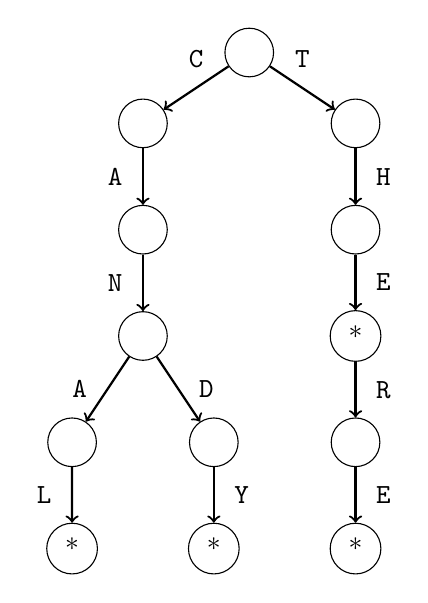
\begin{tikzpicture}[scale=0.9]
\node[draw, circle] (1) at (0,20) {$\phantom{1}$};
\node[draw, circle] (2) at (-1.5,19) {$\phantom{1}$};
\node[draw, circle] (3) at (1.5,19) {$\phantom{1}$};
\node[draw, circle] (4) at (-1.5,17.5) {$\phantom{1}$};
\node[draw, circle] (5) at (-1.5,16) {$\phantom{1}$};
\node[draw, circle] (6) at (-2.5,14.5) {$\phantom{1}$};
\node[draw, circle] (7) at (-0.5,14.5) {$\phantom{1}$};
\node[draw, circle] (8) at (-2.5,13) {*};
\node[draw, circle] (9) at (-0.5,13) {*};
\node[draw, circle] (10) at (1.5,17.5) {$\phantom{1}$};
\node[draw, circle] (11) at (1.5,16) {*};
\node[draw, circle] (12) at (1.5,14.5) {$\phantom{1}$};
\node[draw, circle] (13) at (1.5,13) {*};

\path[draw,thick,->] (1) -- node[font=\small,label=\texttt{C}] {} (2);
\path[draw,thick,->] (1) -- node[font=\small,label=\texttt{T}] {} (3);
\path[draw,thick,->] (2) -- node[font=\small,label=left:\texttt{A}] {} (4);
\path[draw,thick,->] (4) -- node[font=\small,label=left:\texttt{N}] {} (5);
\path[draw,thick,->] (5) -- node[font=\small,label=left:\texttt{A}] {} (6);
\path[draw,thick,->] (5) -- node[font=\small,label=right:\texttt{D}] {} (7);
\path[draw,thick,->] (6) -- node[font=\small,label=left:\texttt{L}] {}(8);
\path[draw,thick,->] (7) -- node[font=\small,label=right:\texttt{Y}] {} (9);
\path[draw,thick,->] (3) -- node[font=\small,label=right:\texttt{H}] {} (10);
\path[draw,thick,->] (10) -- node[font=\small,label=right:\texttt{E}] {} (11);
\path[draw,thick,->] (11) -- node[font=\small,label=right:\texttt{R}] {} (12);
\path[draw,thick,->] (12) -- node[font=\small,label=right:\texttt{E}] {} (13);
\end{tikzpicture}
\end{center}

Cây trie này tương ứng với tập hợp
$\{\texttt{CANAL},\texttt{CANDY},\texttt{THE},\texttt{THERE}\}$.
Ký tự * trong một nút có nghĩa là
một chuỗi trong tập hợp kết thúc tại nút đó.
Một ký tự như vậy là cần thiết, bởi vì một chuỗi
có thể là một tiền tố của một chuỗi khác.
Ví dụ, trong cây trie trên, \texttt{THE}
là một tiền tố của \texttt{THERE}.

Chúng ta có thể kiểm tra trong thời gian $O(n)$ xem một cây trie
có chứa một chuỗi có độ dài $n$ hay không,
bởi vì chúng ta có thể đi theo chuỗi bắt đầu từ nút gốc.
Chúng ta cũng có thể thêm một chuỗi có độ dài $n$ vào cây trie
trong thời gian $O(n)$ bằng cách đi theo chuỗi trước
và sau đó thêm các nút mới vào cây nếu cần.

Sử dụng cây trie, chúng ta có thể tìm
tiền tố dài nhất của một chuỗi cho trước
sao cho tiền tố đó thuộc tập hợp.
Hơn nữa, bằng cách lưu trữ thêm thông tin
trong mỗi nút,
chúng ta có thể tính số lượng
chuỗi thuộc tập hợp và có một
chuỗi cho trước làm tiền tố.

Một cây trie có thể được lưu trữ trong một mảng
\begin{lstlisting}
int trie[N][A];
\end{lstlisting}
trong đó $N$ là số nút tối đa
(tổng độ dài tối đa của các chuỗi trong tập hợp)
và $A$ là kích thước của bảng chữ cái.
Các nút của một cây trie được đánh số
$0,1,2,\ldots$ sao cho số của gốc là 0,
và $\texttt{trie}[s][c]$ là nút tiếp theo trong chuỗi
khi chúng ta di chuyển từ nút $s$ bằng ký tự $c$.

\section{Băm chuỗi (String hashing)}

\index{hashing}
\index{string hashing}

\key{Băm chuỗi (String hashing)} là một kỹ thuật
cho phép chúng ta kiểm tra hiệu quả xem hai
chuỗi có bằng nhau không\footnote{Kỹ thuật
này đã được phổ biến bởi thuật toán khớp mẫu Karp–Rabin \cite{kar87}.}.
Ý tưởng trong băm chuỗi là so sánh các giá trị băm của
các chuỗi thay vì các ký tự riêng lẻ của chúng.

\subsubsection*{Tính giá trị băm}

\index{hash value}
\index{polynomial hashing}

Một \key{giá trị băm (hash value)} của một chuỗi là
một số được tính từ các ký tự
của chuỗi.
Nếu hai chuỗi giống nhau,
các giá trị băm của chúng cũng giống nhau,
điều này cho phép so sánh các chuỗi
dựa trên giá trị băm của chúng.

Một cách thông thường để thực hiện băm chuỗi
là \key{băm đa thức (polynomial hashing)}, có nghĩa là
giá trị băm của một chuỗi \texttt{s}
có độ dài $n$ là
\[(\texttt{s}[0] A^{n-1} + \texttt{s}[1] A^{n-2} + \cdots + \texttt{s}[n-1] A^0) \bmod B  ,\]
trong đó $s[0],s[1],\ldots,s[n-1]$
được hiểu là mã của các ký tự của \texttt{s},
và $A$ và $B$ là các hằng số được chọn trước.

Ví dụ, mã của các ký tự
của \texttt{ALLEY} là:
\begin{center}
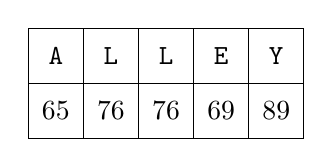
\begin{tikzpicture}[scale=0.7]
\draw (0,0) grid (5,2);

\node at (0.5, 1.5) {\texttt{A}};
\node at (1.5, 1.5) {\texttt{L}};
\node at (2.5, 1.5) {\texttt{L}};
\node at (3.5, 1.5) {\texttt{E}};
\node at (4.5, 1.5) {\texttt{Y}};

\node at (0.5, 0.5) {65};
\node at (1.5, 0.5) {76};
\node at (2.5, 0.5) {76};
\node at (3.5, 0.5) {69};
\node at (4.5, 0.5) {89};

\end{tikzpicture}
\end{center}

Do đó, nếu $A=3$ và $B=97$, giá trị băm
của \texttt{ALLEY} là
\[(65 \cdot 3^4 + 76 \cdot 3^3 + 76 \cdot 3^2 + 69 \cdot 3^1 + 89 \cdot 3^0) \bmod 97 = 52.\]

\subsubsection*{Tiền xử lý}

Sử dụng băm đa thức, chúng ta có thể tính giá trị băm của bất kỳ chuỗi con nào
của một chuỗi \texttt{s} trong thời gian $O(1)$ sau một lần tiền xử lý thời gian $O(n)$.
Ý tưởng là xây dựng một mảng \texttt{h} sao cho
$\texttt{h}[k]$ chứa giá trị băm của tiền tố $\texttt{s}[0 \ldots k]$.
Các giá trị mảng có thể được tính đệ quy như sau:
\[
\begin{array}{lcl}
\texttt{h}[0] & = & \texttt{s}[0] \\
\texttt{h}[k] & = & (\texttt{h}[k-1] A + \texttt{s}[k]) \bmod B \\
\end{array}
\]
Ngoài ra, chúng ta xây dựng một mảng $\texttt{p}$
trong đó $\texttt{p}[k]=A^k \bmod B$:
\[
\begin{array}{lcl}
\texttt{p}[0] & = & 1 \\
\texttt{p}[k] & = & (\texttt{p}[k-1] A) \bmod B. \\
\end{array}
\]
Việc xây dựng các mảng này mất thời gian $O(n)$.
Sau đó, giá trị băm của bất kỳ chuỗi con nào
$\texttt{s}[a \ldots b]$
có thể được tính trong thời gian $O(1)$ bằng công thức
\[(\texttt{h}[b]-\texttt{h}[a-1] \texttt{p}[b-a+1]) \bmod B\]
giả sử rằng $a>0$.
Nếu $a=0$, giá trị băm đơn giản là $\texttt{h}[b]$.

\subsubsection*{Sử dụng giá trị băm}

Chúng ta có thể so sánh các chuỗi một cách hiệu quả bằng cách sử dụng giá trị băm.
Thay vì so sánh các ký tự riêng lẻ của các chuỗi,
ý tưởng là so sánh các giá trị băm của chúng.
Nếu các giá trị băm bằng nhau,
các chuỗi \emph{có thể} bằng nhau,
và nếu các giá trị băm khác nhau,
các chuỗi \emph{chắc chắn} khác nhau.

Sử dụng băm, chúng ta thường có thể làm cho một thuật toán
duyệt toàn bộ trở nên hiệu quả.
Ví dụ, hãy xem xét bài toán khớp mẫu:
cho một chuỗi $s$ và một mẫu $p$,
tìm các vị trí mà $p$ xuất hiện trong $s$.
Một thuật toán duyệt toàn bộ sẽ duyệt qua tất cả các vị trí
mà $p$ có thể xuất hiện và so sánh các chuỗi
từng ký tự một.
Độ phức tạp thời gian của một thuật toán như vậy là $O(n^2)$.

Chúng ta có thể làm cho thuật toán duyệt toàn bộ hiệu quả hơn
bằng cách sử dụng băm, bởi vì thuật toán so sánh
các chuỗi con của các chuỗi.
Sử dụng băm, mỗi phép so sánh chỉ mất thời gian $O(1)$,
bởi vì chỉ có giá trị băm của các chuỗi con được so sánh.
Điều này dẫn đến một thuật toán có độ phức tạp thời gian là $O(n)$,
là độ phức tạp thời gian tốt nhất có thể cho bài toán này.

Bằng cách kết hợp băm và \emph{tìm kiếm nhị phân (binary search)},
cũng có thể tìm ra thứ tự từ điển của
hai chuỗi trong thời gian logarit.
Điều này có thể được thực hiện bằng cách tính độ dài
của tiền tố chung của các chuỗi bằng tìm kiếm nhị phân.
Một khi chúng ta biết độ dài của tiền tố chung,
chúng ta chỉ cần kiểm tra ký tự tiếp theo sau tiền tố,
bởi vì điều này xác định thứ tự của các chuỗi.

\subsubsection*{Xung đột và tham số}

\index{collision}

Một rủi ro rõ ràng khi so sánh các giá trị băm là
một \key{xung đột (collision)}, có nghĩa là hai chuỗi có
nội dung khác nhau nhưng giá trị băm bằng nhau.
Trong trường hợp này, một thuật toán dựa trên
các giá trị băm kết luận rằng các chuỗi bằng nhau,
nhưng thực tế chúng không phải vậy,
và thuật toán có thể cho kết quả không chính xác.

Xung đột luôn có thể xảy ra,
bởi vì số lượng các chuỗi khác nhau lớn hơn
số lượng các giá trị băm khác nhau.
Tuy nhiên, xác suất xảy ra xung đột là nhỏ
nếu các hằng số $A$ và $B$ được chọn cẩn thận.
Một cách thông thường là chọn các hằng số ngẫu nhiên
gần $10^9$, ví dụ như sau:
\[
\begin{array}{lcl}
A & = & 911382323 \\
B & = & 972663749 \\
\end{array}
\]

Sử dụng các hằng số như vậy,
kiểu \texttt{long long} có thể được sử dụng
khi tính toán các giá trị băm,
bởi vì các tích $AB$ và $BB$ sẽ vừa với \texttt{long long}.
Nhưng liệu có đủ để có khoảng $10^9$ giá trị băm khác nhau không?

Hãy xem xét ba kịch bản mà băm có thể được sử dụng:

\textit{Kịch bản 1:} Chuỗi $x$ và $y$ được so sánh với
nhau.
Xác suất xảy ra xung đột là $1/B$ giả sử rằng
tất cả các giá trị băm đều có khả năng xảy ra như nhau.

\textit{Kịch bản 2:} Một chuỗi $x$ được so sánh với các chuỗi
$y_1,y_2,\ldots,y_n$.
Xác suất của một hoặc nhiều xung đột là

\[1-(1-\frac{1}{B})^n.\]

\textit{Kịch bản 3:} Tất cả các cặp chuỗi $x_1,x_2,\ldots,x_n$
được so sánh với nhau.
Xác suất của một hoặc nhiều xung đột là
\[ 1 - \frac{B \cdot (B-1) \cdot (B-2) \cdots (B-n+1)}{B^n}.\]

Bảng sau cho thấy xác suất xung đột
khi $n=10^6$ và giá trị của $B$ thay đổi:

\begin{center}
\begin{tabular}{rrrr}
hằng số $B$ & kịch bản 1 & kịch bản 2 & kịch bản 3 \\
\hline
$10^3$ & $0.001000$ & $1.000000$ & $1.000000$ \\
$10^6$ & $0.000001$ & $0.632121$ & $1.000000$ \\
$10^9$ & $0.000000$ & $0.001000$ & $1.000000$ \\
$10^{12}$ & $0.000000$ & $0.000000$ & $0.393469$ \\
$10^{15}$ & $0.000000$ & $0.000000$ & $0.000500$ \\
$10^{18}$ & $0.000000$ & $0.000000$ & $0.000001$ \\
\end{tabular}
\end{center}

Bảng cho thấy rằng trong kịch bản 1,
xác suất xảy ra xung đột là không đáng kể
khi $B \approx 10^9$.
Trong kịch bản 2, một xung đột có thể xảy ra nhưng
xác suất vẫn khá nhỏ.
Tuy nhiên, trong kịch bản 3, tình hình rất khác:
một xung đột gần như luôn luôn xảy ra khi
$B \approx 10^9$.

\index{birthday paradox}

Hiện tượng trong kịch bản 3 được biết đến với tên gọi
\key{nghịch lý ngày sinh (birthday paradox)}: nếu có $n$ người
trong một căn phòng, xác suất để \emph{một vài} hai người
có cùng ngày sinh là lớn ngay cả khi $n$ khá nhỏ.
Tương ứng, trong băm, khi tất cả các giá trị băm được so sánh
với nhau, xác suất để một vài hai
giá trị băm bằng nhau là lớn.

Chúng ta có thể làm cho xác suất xảy ra xung đột
nhỏ hơn bằng cách tính \emph{nhiều} giá trị băm
sử dụng các tham số khác nhau.
Không có khả năng một xung đột sẽ xảy ra
ở tất cả các giá trị băm cùng một lúc.
Ví dụ, hai giá trị băm với tham số
$B \approx 10^9$ tương ứng với một giá trị
băm với tham số $B \approx 10^{18}$,
điều này làm cho xác suất xảy ra xung đột rất nhỏ.

Một số người sử dụng các hằng số $B=2^{32}$ và $B=2^{64}$,
điều này thuận tiện, bởi vì các phép toán với các số nguyên 32 và 64
bit được tính theo modulo $2^{32}$ và $2^{64}$.
Tuy nhiên, đây \emph{không phải} là một lựa chọn tốt, bởi vì có thể
xây dựng các đầu vào luôn tạo ra xung đột khi
các hằng số có dạng $2^x$ được sử dụng \cite{pac13}.

\section{Thuật toán Z (Z-algorithm)}

\index{Z-algorithm}
\index{Z-array}

\key{Mảng Z (Z-array)} \texttt{z} của một chuỗi \texttt{s}
có độ dài $n$ chứa cho mỗi $k=0,1,\ldots,n-1$
độ dài của chuỗi con dài nhất của \texttt{s}
bắt đầu tại vị trí $k$ và là một tiền tố của \texttt{s}.
Do đó, $\texttt{z}[k]=p$ cho chúng ta biết rằng
$\texttt{s}[0 \ldots p-1]$ bằng $\texttt{s}[k \ldots k+p-1]$.
Nhiều bài toán xử lý chuỗi có thể được giải quyết hiệu quả
bằng cách sử dụng mảng Z.

Ví dụ, mảng Z của
\texttt{ACBACDACBACBACDA} như sau:

\begin{center}
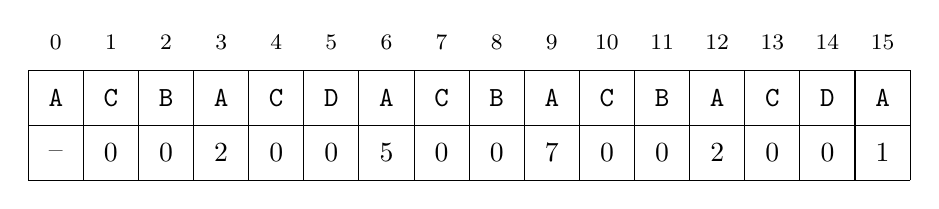
\begin{tikzpicture}[scale=0.7]
\draw (0,0) grid (16,2);

\node at (0.5, 1.5) {\texttt{A}};
\node at (1.5, 1.5) {\texttt{C}};
\node at (2.5, 1.5) {\texttt{B}};
\node at (3.5, 1.5) {\texttt{A}};
\node at (4.5, 1.5) {\texttt{C}};
\node at (5.5, 1.5) {\texttt{D}};
\node at (6.5, 1.5) {\texttt{A}};
\node at (7.5, 1.5) {\texttt{C}};
\node at (8.5, 1.5) {\texttt{B}};
\node at (9.5, 1.5) {\texttt{A}};
\node at (10.5, 1.5) {\texttt{C}};
\node at (11.5, 1.5) {\texttt{B}};
\node at (12.5, 1.5) {\texttt{A}};
\node at (13.5, 1.5) {\texttt{C}};
\node at (14.5, 1.5) {\texttt{D}};
\node at (15.5, 1.5) {\texttt{A}};

\node at (0.5, 0.5) {--};
\node at (1.5, 0.5) {0};
\node at (2.5, 0.5) {0};
\node at (3.5, 0.5) {2};
\node at (4.5, 0.5) {0};
\node at (5.5, 0.5) {0};
\node at (6.5, 0.5) {5};
\node at (7.5, 0.5) {0};
\node at (8.5, 0.5) {0};
\node at (9.5, 0.5) {7};
\node at (10.5, 0.5) {0};
\node at (11.5, 0.5) {0};
\node at (12.5, 0.5) {2};
\node at (13.5, 0.5) {0};
\node at (14.5, 0.5) {0};
\node at (15.5, 0.5) {1};

\footnotesize
\node at (0.5, 2.5) {0};
\node at (1.5, 2.5) {1};
\node at (2.5, 2.5) {2};
\node at (3.5, 2.5) {3};
\node at (4.5, 2.5) {4};
\node at (5.5, 2.5) {5};
\node at (6.5, 2.5) {6};
\node at (7.5, 2.5) {7};
\node at (8.5, 2.5) {8};
\node at (9.5, 2.5) {9};
\node at (10.5, 2.5) {10};
\node at (11.5, 2.5) {11};
\node at (12.5, 2.5) {12};
\node at (13.5, 2.5) {13};
\node at (14.5, 2.5) {14};
\node at (15.5, 2.5) {15};

\end{tikzpicture}
\end{center}

Trong trường hợp này, ví dụ, $\texttt{z}[6]=5$,
bởi vì chuỗi con \texttt{ACBAC} có độ dài 5
là một tiền tố của \texttt{s},
nhưng chuỗi con \texttt{ACBACB} có độ dài 6
không phải là một tiền tố của \texttt{s}.

\subsubsection*{Mô tả thuật toán}

Tiếp theo chúng ta mô tả một thuật toán,
được gọi là \key{thuật toán Z (Z-algorithm)}\footnote{Thuật toán Z
được trình bày trong \cite{gus97} là phương pháp đơn giản nhất được biết đến
cho việc khớp mẫu trong thời gian tuyến tính, và ý tưởng ban đầu
được cho là của \cite{mai84}.},
xây dựng mảng Z một cách hiệu quả trong thời gian $O(n)$.
Thuật toán tính toán các giá trị mảng Z
từ trái sang phải bằng cách vừa sử dụng thông tin
đã được lưu trữ trong mảng Z vừa so sánh các chuỗi con
từng ký tự một.

Để tính toán hiệu quả các giá trị mảng Z,
thuật toán duy trì một khoảng $[x,y]$ sao cho
$\texttt{s}[x \ldots y]$ là một tiền tố của \texttt{s}
và $y$ lớn nhất có thể.
Vì chúng ta biết rằng $\texttt{s}[0 \ldots y-x]$
và $\texttt{s}[x \ldots y]$ bằng nhau,
chúng ta có thể sử dụng thông tin này khi tính
các giá trị Z cho các vị trí $x+1,x+2,\ldots,y$.

Tại mỗi vị trí $k$, chúng ta trước tiên
kiểm tra giá trị của $\texttt{z}[k-x]$.
Nếu $k+\texttt{z}[k-x]<y$, chúng ta biết rằng $\texttt{z}[k]=\texttt{z}[k-x]$.
Tuy nhiên, nếu $k+\texttt{z}[k-x] \ge y$,
$\texttt{s}[0 \ldots y-k]$ bằng
$\texttt{s}[k \ldots y]$, và để xác định
giá trị của $\texttt{z}[k]$ chúng ta cần so sánh
các chuỗi con từng ký tự một.
Tuy nhiên, thuật toán vẫn hoạt động trong thời gian $O(n)$,
bởi vì chúng ta bắt đầu so sánh tại các vị trí
$y-k+1$ và $y+1$.

Ví dụ, chúng ta hãy xây dựng mảng Z sau:

\begin{center}
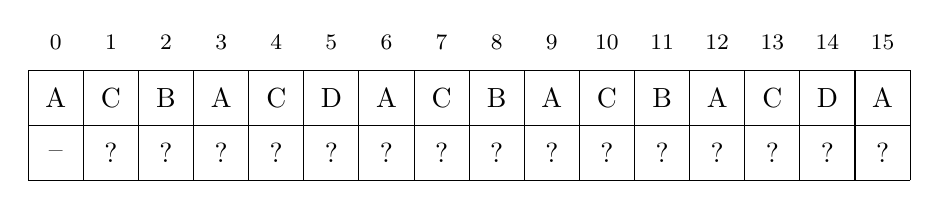
\begin{tikzpicture}[scale=0.7]
\draw (0,0) grid (16,2);

\node at (0.5, 1.5) {A};
\node at (1.5, 1.5) {C};
\node at (2.5, 1.5) {B};
\node at (3.5, 1.5) {A};
\node at (4.5, 1.5) {C};
\node at (5.5, 1.5) {D};
\node at (6.5, 1.5) {A};
\node at (7.5, 1.5) {C};
\node at (8.5, 1.5) {B};
\node at (9.5, 1.5) {A};
\node at (10.5, 1.5) {C};
\node at (11.5, 1.5) {B};
\node at (12.5, 1.5) {A};
\node at (13.5, 1.5) {C};
\node at (14.5, 1.5) {D};
\node at (15.5, 1.5) {A};

\node at (0.5, 0.5) {--};
\node at (1.5, 0.5) {?};
\node at (2.5, 0.5) {?};
\node at (3.5, 0.5) {?};
\node at (4.5, 0.5) {?};
\node at (5.5, 0.5) {?};
\node at (6.5, 0.5) {?};
\node at (7.5, 0.5) {?};
\node at (8.5, 0.5) {?};
\node at (9.5, 0.5) {?};
\node at (10.5, 0.5) {?};
\node at (11.5, 0.5) {?};
\node at (12.5, 0.5) {?};
\node at (13.5, 0.5) {?};
\node at (14.5, 0.5) {?};
\node at (15.5, 0.5) {?};

\footnotesize
\node at (0.5, 2.5) {0};
\node at (1.5, 2.5) {1};
\node at (2.5, 2.5) {2};
\node at (3.5, 2.5) {3};
\node at (4.5, 2.5) {4};
\node at (5.5, 2.5) {5};
\node at (6.5, 2.5) {6};
\node at (7.5, 2.5) {7};
\node at (8.5, 2.5) {8};
\node at (9.5, 2.5) {9};
\node at (10.5, 2.5) {10};
\node at (11.5, 2.5) {11};
\node at (12.5, 2.5) {12};
\node at (13.5, 2.5) {13};
\node at (14.5, 2.5) {14};
\node at (15.5, 2.5) {15};

\end{tikzpicture}
\end{center}

Sau khi tính giá trị $\texttt{z}[6]=5$,
khoảng $[x,y]$ hiện tại là $[6,10]$:

\begin{center}
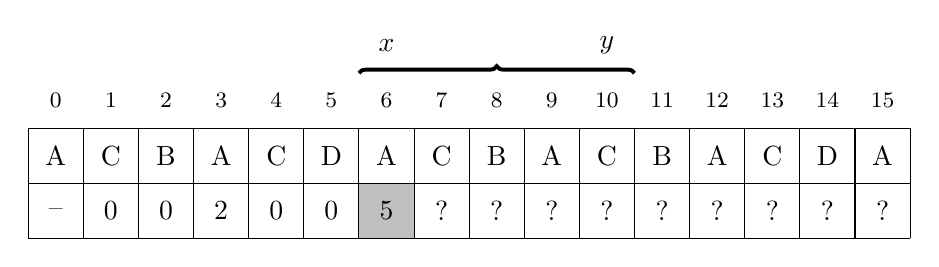
\begin{tikzpicture}[scale=0.7]
\fill[color=lightgray] (6,0) rectangle (7,1);
\draw (0,0) grid (16,2);

\node at (0.5, 1.5) {A};
\node at (1.5, 1.5) {C};
\node at (2.5, 1.5) {B};
\node at (3.5, 1.5) {A};
\node at (4.5, 1.5) {C};
\node at (5.5, 1.5) {D};
\node at (6.5, 1.5) {A};
\node at (7.5, 1.5) {C};
\node at (8.5, 1.5) {B};
\node at (9.5, 1.5) {A};
\node at (10.5, 1.5) {C};
\node at (11.5, 1.5) {B};
\node at (12.5, 1.5) {A};
\node at (13.5, 1.5) {C};
\node at (14.5, 1.5) {D};
\node at (15.5, 1.5) {A};

\node at (0.5, 0.5) {--};
\node at (1.5, 0.5) {0};
\node at (2.5, 0.5) {0};
\node at (3.5, 0.5) {2};
\node at (4.5, 0.5) {0};
\node at (5.5, 0.5) {0};
\node at (6.5, 0.5) {5};
\node at (7.5, 0.5) {?};
\node at (8.5, 0.5) {?};
\node at (9.5, 0.5) {?};
\node at (10.5, 0.5) {?};
\node at (11.5, 0.5) {?};
\node at (12.5, 0.5) {?};
\node at (13.5, 0.5) {?};
\node at (14.5, 0.5) {?};
\node at (15.5, 0.5) {?};

\draw [decoration={brace}, decorate, line width=0.5mm] (6,3.00) -- (11,3.00);

\node at (6.5,3.50) {$x$};
\node at (10.5,3.50) {$y$};


\footnotesize
\node at (0.5, 2.5) {0};
\node at (1.5, 2.5) {1};
\node at (2.5, 2.5) {2};
\node at (3.5, 2.5) {3};
\node at (4.5, 2.5) {4};
\node at (5.5, 2.5) {5};
\node at (6.5, 2.5) {6};
\node at (7.5, 2.5) {7};
\node at (8.5, 2.5) {8};
\node at (9.5, 2.5) {9};
\node at (10.5, 2.5) {10};
\node at (11.5, 2.5) {11};
\node at (12.5, 2.5) {12};
\node at (13.5, 2.5) {13};
\node at (14.5, 2.5) {14};
\node at (15.5, 2.5) {15};

\end{tikzpicture}
\end{center}

Bây giờ chúng ta có thể tính
các giá trị mảng Z tiếp theo
một cách hiệu quả,
bởi vì chúng ta biết rằng
$\texttt{s}[0 \ldots 4]$ và
$\texttt{s}[6 \ldots 10]$ bằng nhau.
Đầu tiên, vì $\texttt{z}[1] = \texttt{z}[2] = 0$,
chúng ta ngay lập tức biết rằng cũng
$\texttt{z}[7] = \texttt{z}[8] = 0$:

\begin{center}
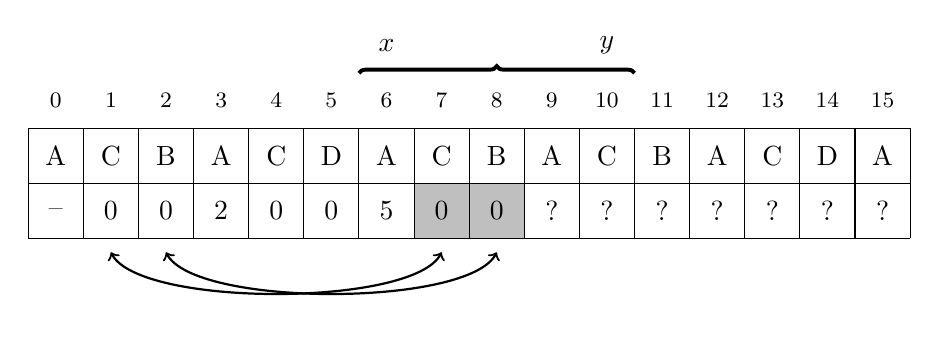
\begin{tikzpicture}[scale=0.7]
\fill[color=lightgray] (7,0) rectangle (9,1);
\draw (0,0) grid (16,2);

\node at (0.5, 1.5) {A};
\node at (1.5, 1.5) {C};
\node at (2.5, 1.5) {B};
\node at (3.5, 1.5) {A};
\node at (4.5, 1.5) {C};
\node at (5.5, 1.5) {D};
\node at (6.5, 1.5) {A};
\node at (7.5, 1.5) {C};
\node at (8.5, 1.5) {B};
\node at (9.5, 1.5) {A};
\node at (10.5, 1.5) {C};
\node at (11.5, 1.5) {B};
\node at (12.5, 1.5) {A};
\node at (13.5, 1.5) {C};
\node at (14.5, 1.5) {D};
\node at (15.5, 1.5) {A};

\node at (0.5, 0.5) {--};
\node at (1.5, 0.5) {0};
\node at (2.5, 0.5) {0};
\node at (3.5, 0.5) {2};
\node at (4.5, 0.5) {0};
\node at (5.5, 0.5) {0};
\node at (6.5, 0.5) {5};
\node at (7.5, 0.5) {0};
\node at (8.5, 0.5) {0};
\node at (9.5, 0.5) {?};
\node at (10.5, 0.5) {?};
\node at (11.5, 0.5) {?};
\node at (12.5, 0.5) {?};
\node at (13.5, 0.5) {?};
\node at (14.5, 0.5) {?};
\node at (15.5, 0.5) {?};


\draw [decoration={brace}, decorate, line width=0.5mm] (6,3.00) -- (11,3.00);

\node at (6.5,3.50) {$x$};
\node at (10.5,3.50) {$y$};


\footnotesize
\node at (0.5, 2.5) {0};
\node at (1.5, 2.5) {1};
\node at (2.5, 2.5) {2};
\node at (3.5, 2.5) {3};
\node at (4.5, 2.5) {4};
\node at (5.5, 2.5) {5};
\node at (6.5, 2.5) {6};
\node at (7.5, 2.5) {7};
\node at (8.5, 2.5) {8};
\node at (9.5, 2.5) {9};
\node at (10.5, 2.5) {10};
\node at (11.5, 2.5) {11};
\node at (12.5, 2.5) {12};
\node at (13.5, 2.5) {13};
\node at (14.5, 2.5) {14};
\node at (15.5, 2.5) {15};


\draw[thick,<->] (7.5,-0.25) .. controls (7,-1.25) and (2,-1.25) .. (1.5,-0.25);
\draw[thick,<->] (8.5,-0.25) .. controls (8,-1.25) and (3,-1.25) .. (2.5,-0.25);
\end{tikzpicture}
\end{center}

Sau đó, vì $\texttt{z}[3]=2$, chúng ta biết rằng $\texttt{z}[9] \ge 2$:

\begin{center}
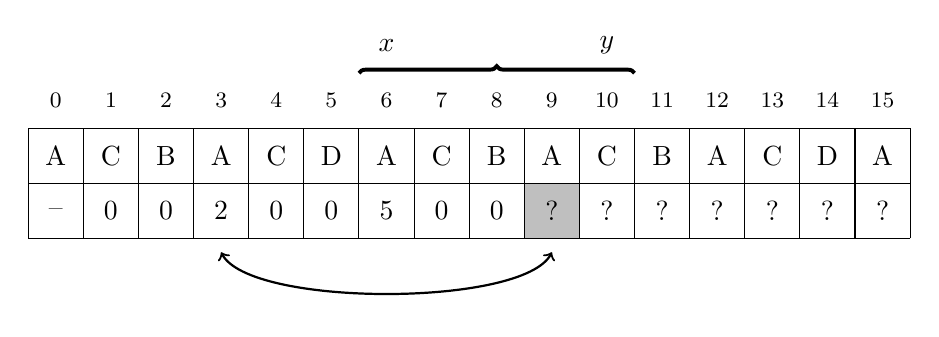
\begin{tikzpicture}[scale=0.7]
\fill[color=lightgray] (9,0) rectangle (10,1);
\draw (0,0) grid (16,2);

\node at (0.5, 1.5) {A};
\node at (1.5, 1.5) {C};
\node at (2.5, 1.5) {B};
\node at (3.5, 1.5) {A};
\node at (4.5, 1.5) {C};
\node at (5.5, 1.5) {D};
\node at (6.5, 1.5) {A};
\node at (7.5, 1.5) {C};
\node at (8.5, 1.5) {B};
\node at (9.5, 1.5) {A};
\node at (10.5, 1.5) {C};
\node at (11.5, 1.5) {B};
\node at (12.5, 1.5) {A};
\node at (13.5, 1.5) {C};
\node at (14.5, 1.5) {D};
\node at (15.5, 1.5) {A};

\node at (0.5, 0.5) {--};
\node at (1.5, 0.5) {0};
\node at (2.5, 0.5) {0};
\node at (3.5, 0.5) {2};
\node at (4.5, 0.5) {0};
\node at (5.5, 0.5) {0};
\node at (6.5, 0.5) {5};
\node at (7.5, 0.5) {0};
\node at (8.5, 0.5) {0};
\node at (9.5, 0.5) {?};
\node at (10.5, 0.5) {?};
\node at (11.5, 0.5) {?};
\node at (12.5, 0.5) {?};
\node at (13.5, 0.5) {?};
\node at (14.5, 0.5) {?};
\node at (15.5, 0.5) {?};

\draw [decoration={brace}, decorate, line width=0.5mm] (6,3.00) -- (11,3.00);

\node at (6.5,3.50) {$x$};
\node at (10.5,3.50) {$y$};


\footnotesize
\node at (0.5, 2.5) {0};
\node at (1.5, 2.5) {1};
\node at (2.5, 2.5) {2};
\node at (3.5, 2.5) {3};
\node at (4.5, 2.5) {4};
\node at (5.5, 2.5) {5};
\node at (6.5, 2.5) {6};
\node at (7.5, 2.5) {7};
\node at (8.5, 2.5) {8};
\node at (9.5, 2.5) {9};
\node at (10.5, 2.5) {10};
\node at (11.5, 2.5) {11};
\node at (12.5, 2.5) {12};
\node at (13.5, 2.5) {13};
\node at (14.5, 2.5) {14};
\node at (15.5, 2.5) {15};

\draw[thick,<->] (9.5,-0.25) .. controls (9,-1.25) and (4,-1.25) .. (3.5,-0.25);
\end{tikzpicture}
\end{center}

Tuy nhiên, chúng ta không có thông tin về chuỗi
sau vị trí 10, vì vậy chúng ta cần so sánh các chuỗi con
từng ký tự một:

\begin{center}
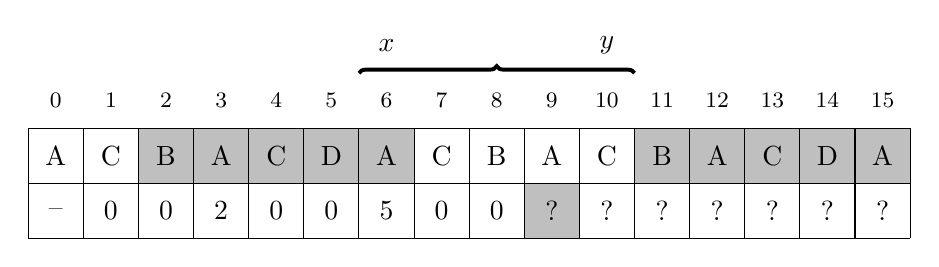
\begin{tikzpicture}[scale=0.7]
\fill[color=lightgray] (9,0) rectangle (10,1);
\fill[color=lightgray] (2,1) rectangle (7,2);
\fill[color=lightgray] (11,1) rectangle (16,2);


\draw (0,0) grid (16,2);

\node at (0.5, 1.5) {A};
\node at (1.5, 1.5) {C};
\node at (2.5, 1.5) {B};
\node at (3.5, 1.5) {A};
\node at (4.5, 1.5) {C};
\node at (5.5, 1.5) {D};
\node at (6.5, 1.5) {A};
\node at (7.5, 1.5) {C};
\node at (8.5, 1.5) {B};
\node at (9.5, 1.5) {A};
\node at (10.5, 1.5) {C};
\node at (11.5, 1.5) {B};
\node at (12.5, 1.5) {A};
\node at (13.5, 1.5) {C};
\node at (14.5, 1.5) {D};
\node at (15.5, 1.5) {A};

\node at (0.5, 0.5) {--};
\node at (1.5, 0.5) {0};
\node at (2.5, 0.5) {0};
\node at (3.5, 0.5) {2};
\node at (4.5, 0.5) {0};
\node at (5.5, 0.5) {0};
\node at (6.5, 0.5) {5};
\node at (7.5, 0.5) {0};
\node at (8.5, 0.5) {0};
\node at (9.5, 0.5) {?};
\node at (10.5, 0.5) {?};
\node at (11.5, 0.5) {?};
\node at (12.5, 0.5) {?};
\node at (13.5, 0.5) {?};
\node at (14.5, 0.5) {?};
\node at (15.5, 0.5) {?};

\draw [decoration={brace}, decorate, line width=0.5mm] (6,3.00) -- (11,3.00);

\node at (6.5,3.50) {$x$};
\node at (10.5,3.50) {$y$};


\footnotesize
\node at (0.5, 2.5) {0};
\node at (1.5, 2.5) {1};
\node at (2.5, 2.5) {2};
\node at (3.5, 2.5) {3};
\node at (4.5, 2.5) {4};
\node at (5.5, 2.5) {5};
\node at (6.5, 2.5) {6};
\node at (7.5, 2.5) {7};
\node at (8.5, 2.5) {8};
\node at (9.5, 2.5) {9};
\node at (10.5, 2.5) {10};
\node at (11.5, 2.5) {11};
\node at (12.5, 2.5) {12};
\node at (13.5, 2.5) {13};
\node at (14.5, 2.5) {14};
\node at (15.5, 2.5) {15};

\end{tikzpicture}
\end{center}

Hóa ra $\texttt{z}[9]=7$,
vì vậy khoảng $[x,y]$ mới là $[9,15]$:

\begin{center}
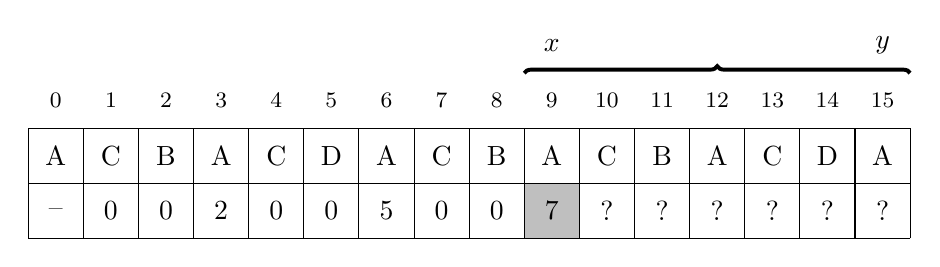
\begin{tikzpicture}[scale=0.7]
\fill[color=lightgray] (9,0) rectangle (10,1);
\draw (0,0) grid (16,2);

\node at (0.5, 1.5) {A};
\node at (1.5, 1.5) {C};
\node at (2.5, 1.5) {B};
\node at (3.5, 1.5) {A};
\node at (4.5, 1.5) {C};
\node at (5.5, 1.5) {D};
\node at (6.5, 1.5) {A};
\node at (7.5, 1.5) {C};
\node at (8.5, 1.5) {B};
\node at (9.5, 1.5) {A};
\node at (10.5, 1.5) {C};
\node at (11.5, 1.5) {B};
\node at (12.5, 1.5) {A};
\node at (13.5, 1.5) {C};
\node at (14.5, 1.5) {D};
\node at (15.5, 1.5) {A};

\node at (0.5, 0.5) {--};
\node at (1.5, 0.5) {0};
\node at (2.5, 0.5) {0};
\node at (3.5, 0.5) {2};
\node at (4.5, 0.5) {0};
\node at (5.5, 0.5) {0};
\node at (6.5, 0.5) {5};
\node at (7.5, 0.5) {0};
\node at (8.5, 0.5) {0};
\node at (9.5, 0.5) {7};
\node at (10.5, 0.5) {?};
\node at (11.5, 0.5) {?};
\node at (12.5, 0.5) {?};
\node at (13.5, 0.5) {?};
\node at (14.5, 0.5) {?};
\node at (15.5, 0.5) {?};

\draw [decoration={brace}, decorate, line width=0.5mm] (9,3.00) -- (16,3.00);

\node at (9.5,3.50) {$x$};
\node at (15.5,3.50) {$y$};


\footnotesize
\node at (0.5, 2.5) {0};
\node at (1.5, 2.5) {1};
\node at (2.5, 2.5) {2};
\node at (3.5, 2.5) {3};
\node at (4.5, 2.5) {4};
\node at (5.5, 2.5) {5};
\node at (6.5, 2.5) {6};
\node at (7.5, 2.5) {7};
\node at (8.5, 2.5) {8};
\node at (9.5, 2.5) {9};
\node at (10.5, 2.5) {10};
\node at (11.5, 2.5) {11};
\node at (12.5, 2.5) {12};
\node at (13.5, 2.5) {13};
\node at (14.5, 2.5) {14};
\node at (15.5, 2.5) {15};

\end{tikzpicture}
\end{center}

Sau đó, tất cả các giá trị mảng Z còn lại
có thể được xác định bằng cách sử dụng thông tin
đã được lưu trữ trong mảng Z:

\begin{center}
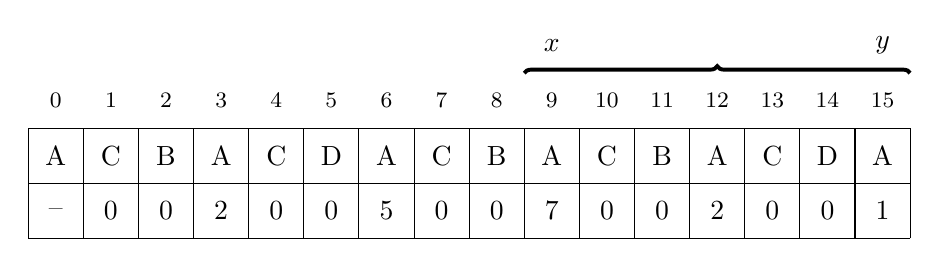
\begin{tikzpicture}[scale=0.7]
\draw (0,0) grid (16,2);

\node at (0.5, 1.5) {A};
\node at (1.5, 1.5) {C};
\node at (2.5, 1.5) {B};
\node at (3.5, 1.5) {A};
\node at (4.5, 1.5) {C};
\node at (5.5, 1.5) {D};
\node at (6.5, 1.5) {A};
\node at (7.5, 1.5) {C};
\node at (8.5, 1.5) {B};
\node at (9.5, 1.5) {A};
\node at (10.5, 1.5) {C};
\node at (11.5, 1.5) {B};
\node at (12.5, 1.5) {A};
\node at (13.5, 1.5) {C};
\node at (14.5, 1.5) {D};
\node at (15.5, 1.5) {A};

\node at (0.5, 0.5) {--};
\node at (1.5, 0.5) {0};
\node at (2.5, 0.5) {0};
\node at (3.5, 0.5) {2};
\node at (4.5, 0.5) {0};
\node at (5.5, 0.5) {0};
\node at (6.5, 0.5) {5};
\node at (7.5, 0.5) {0};
\node at (8.5, 0.5) {0};
\node at (9.5, 0.5) {7};
\node at (10.5, 0.5) {0};
\node at (11.5, 0.5) {0};
\node at (12.5, 0.5) {2};
\node at (13.5, 0.5) {0};
\node at (14.5, 0.5) {0};
\node at (15.5, 0.5) {1};

\draw [decoration={brace}, decorate, line width=0.5mm] (9,3.00) -- (16,3.00);

\node at (9.5,3.50) {$x$};
\node at (15.5,3.50) {$y$};


\footnotesize
\node at (0.5, 2.5) {0};
\node at (1.5, 2.5) {1};
\node at (2.5, 2.5) {2};
\node at (3.5, 2.5) {3};
\node at (4.5, 2.5) {4};
\node at (5.5, 2.5) {5};
\node at (6.5, 2.5) {6};
\node at (7.5, 2.5) {7};
\node at (8.5, 2.5) {8};
\node at (9.5, 2.5) {9};
\node at (10.5, 2.5) {10};
\node at (11.5, 2.5) {11};
\node at (12.5, 2.5) {12};
\node at (13.5, 2.5) {13};
\node at (14.5, 2.5) {14};
\node at (15.5, 2.5) {15};

\end{tikzpicture}
\end{center}

\subsubsection{Sử dụng mảng Z}

Thường thì việc sử dụng
băm chuỗi hay thuật toán Z là tùy thuộc vào sở thích.
Không giống như băm, thuật toán Z luôn hoạt động
và không có nguy cơ xảy ra xung đột.
Mặt khác, thuật toán Z khó thực hiện hơn
và một số bài toán chỉ có thể được giải quyết
bằng cách sử dụng băm.

Ví dụ, hãy xem xét lại
bài toán khớp mẫu,
trong đó nhiệm vụ của chúng ta là tìm các lần xuất hiện
của một mẫu $p$ trong một chuỗi $s$.
Chúng ta đã giải quyết bài toán này một cách hiệu quả
bằng cách sử dụng băm chuỗi, nhưng thuật toán Z
cung cấp một cách khác để giải quyết bài toán.

Một ý tưởng thông thường trong xử lý chuỗi là
xây dựng một chuỗi bao gồm
nhiều chuỗi được phân tách bằng các ký tự đặc biệt.
Trong bài toán này, chúng ta có thể xây dựng một chuỗi
$p$\texttt{\#}$s$,
trong đó $p$ và $s$ được phân tách bằng một ký tự đặc biệt
\texttt{\#} không xuất hiện
trong các chuỗi.
Mảng Z của $p$\texttt{\#}$s$ cho chúng ta biết các vị trí
mà $p$ xuất hiện trong $s$,
bởi vì các vị trí đó chứa độ dài của $p$.

Ví dụ, nếu $s=$\texttt{HATTIVATTI} và $p=$\texttt{ATT},
mảng Z như sau:

\begin{center}
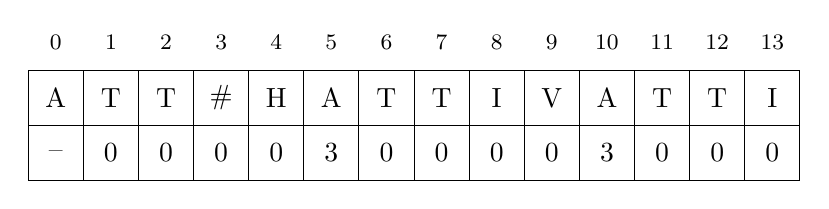
\begin{tikzpicture}[scale=0.7]
\draw (0,0) grid (14,2);

\node at (0.5, 1.5) {A};
\node at (1.5, 1.5) {T};
\node at (2.5, 1.5) {T};
\node at (3.5, 1.5) {\#};
\node at (4.5, 1.5) {H};
\node at (5.5, 1.5) {A};
\node at (6.5, 1.5) {T};
\node at (7.5, 1.5) {T};
\node at (8.5, 1.5) {I};
\node at (9.5, 1.5) {V};
\node at (10.5, 1.5) {A};
\node at (11.5, 1.5) {T};
\node at (12.5, 1.5) {T};
\node at (13.5, 1.5) {I};

\node at (0.5, 0.5) {--};
\node at (1.5, 0.5) {0};
\node at (2.5, 0.5) {0};
\node at (3.5, 0.5) {0};
\node at (4.5, 0.5) {0};
\node at (5.5, 0.5) {3};
\node at (6.5, 0.5) {0};
\node at (7.5, 0.5) {0};
\node at (8.5, 0.5) {0};
\node at (9.5, 0.5) {0};
\node at (10.5, 0.5) {3};
\node at (11.5, 0.5) {0};
\node at (12.5, 0.5) {0};
\node at (13.5, 0.5) {0};

\footnotesize
\node at (0.5, 2.5) {0};
\node at (1.5, 2.5) {1};
\node at (2.5, 2.5) {2};
\node at (3.5, 2.5) {3};
\node at (4.5, 2.5) {4};
\node at (5.5, 2.5) {5};
\node at (6.5, 2.5) {6};
\node at (7.5, 2.5) {7};
\node at (8.5, 2.5) {8};
\node at (9.5, 2.5) {9};
\node at (10.5, 2.5) {10};
\node at (11.5, 2.5) {11};
\node at (12.5, 2.5) {12};
\node at (13.5, 2.5) {13};
\end{tikzpicture}
\end{center}

Các vị trí 5 và 10 chứa giá trị 3,
có nghĩa là mẫu \texttt{ATT}
xuất hiện ở các vị trí tương ứng
của \texttt{HATTIVATTI}.

Độ phức tạp thời gian của thuật toán kết quả
là tuyến tính, bởi vì chỉ cần xây dựng
mảng Z và duyệt qua các giá trị của nó.

\subsubsection{Cài đặt}

Đây là một cài đặt ngắn gọn của thuật toán Z
trả về một vector tương ứng với mảng Z.

\begin{lstlisting}
vector<int> z(string s) {
    int n = s.size();
    vector<int> z(n);
    int x = 0, y = 0;
    for (int i = 1; i < n; i++) {
        z[i] = max(0,min(z[i-x],y-i+1));
        while (i+z[i] < n && s[z[i]] == s[i+z[i]]) {
            x = i; y = i+z[i]; z[i]++;
        }
    }
    return z;
}
\end{lstlisting}